\section{对偶上升}
\label{sec:pm-dual-ascent}

二次罚的解满足$\rho h(\bm{x}_\rho)\to\nu^\star$，一次罚的门槛也是乘子。两节下来，真正需要的量似乎一直是乘子，罚项只是在间接地把它制造出来。本节换一个问题：如果直接把乘子当作价格来调整，不加任何罚项，能走多远？

\paragraph{价格让碗倾斜}
先回到工厂的例子。总部报出乘子$\nu$，相当于对约束$x_1+x_2-4$计价，两家工厂面对的是Lagrange函数：
\[
 \mathcal{L}(\bm{x},\nu)=\frac12x_1^2+\frac32x_2^2+\nu(x_1+x_2-4).
\]
固定$\nu$，这是一个没有约束的严格凸二次函数。令梯度为零，得到
\begin{equation}
 \bm{x}(\nu)=-\nu\Bigl(1,\ \frac13\Bigr).
 \label{eq:pm-running-lagrange-min}
\end{equation}
写成$p=-\nu$更好读：单价$p$越高，工厂产量越高，$x_1=p$，$x_2=p/3$。线性项$\nu(x_1+x_2)$不改变碗的形状，只把碗底平移。

图~\ref{fig:pm-price-tilt}是平移的过程。$\nu=0$时碗底在原点，离约束很远。$\nu=-2.4$时碗底靠近直线，还差一点。$\nu=-3$时碗底恰好落在约束上的红点处，也就是原问题的解。这时不用任何约束，无约束最小点自己满足了约束。

\begin{BookInlineFigure}
  \centering
  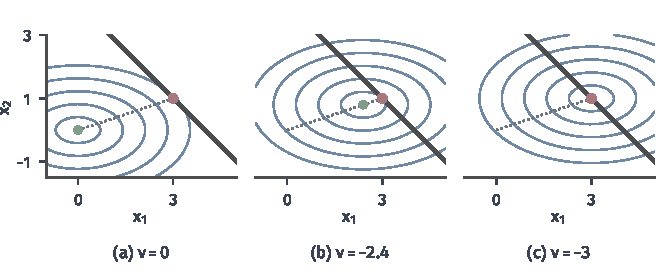
\includegraphics[width=112mm]{figures/05-optimization/06-constrained-optimization/matplotlib/pm-price-tilt/figure.pdf}
  \caption{乘子使Lagrange函数的碗底平移。蓝线是$\mathcal{L}(\cdot,\nu)$的等高线，深灰直线是约束，绿点是$\bm{x}(\nu)$，红点是解$(3,1)$，灰色点线是碗底走过的射线。(c)中$\nu=\nu^\star=-3$，碗底恰好落在约束上。}
  \label{fig:pm-price-tilt}
\end{BookInlineFigure}

把$\bm{x}(\nu)$代回，得到这个例子的对偶函数，它是Lagrange函数在$\bm{x}$上的最小值：
\[
 q(\nu)=\frac12\nu^2+\frac16\nu^2+\nu\Bigl(-\frac43\nu-4\Bigr).
\]
合并同类项，结果是
\begin{equation}
 q(\nu)=-\frac23\nu^2-4\nu .
 \label{eq:pm-running-dual}
\end{equation}
由弱对偶，每个$q(\nu)$都是$f^\star$的下界。这个二次函数在$\nu^\star=-3$处达到最大值$q(-3)=6=f^\star$。

\paragraph{一般情形}
一般问题中，固定$(\bm{\lambda},\bm{\nu})$，要解的是Lagrange子问题。第~\ref{chap:duality}章定义了对偶函数，这里允许把简单的集合$\bm{X}$（如整个空间或盒子）保留在子问题里：
\begin{equation}
 q(\bm{\lambda},\bm{\nu})=\inf_{\bm{x}\in\bm{X}}\mathcal{L}(\bm{x},\bm{\lambda},\bm{\nu}).
 \label{eq:pm-dual-function}
\end{equation}
它是一族关于$(\bm{\lambda},\bm{\nu})$的线性函数的下确界，因此总是凹的，这与原问题是否凸无关。求解对偶问题就是在$\bm{\lambda}\geq\bm{0}$上最大化这个凹函数。

\subsection{残差与乘子更新}
\label{sec:pm-dual-update}

要上升就要知道方向。这里的好消息是：解完Lagrange子问题，约束残差就是现成的上升信息。

\paragraph{残差是超梯度}
二元例的导数是$q'(\nu)=-\tfrac43\nu-4$，把式~\eqref{eq:pm-running-lagrange-min}代入，这恰好等于$h(\bm{x}(\nu))$。一般情形下$q$可能不可微，需要先推广“梯度”。

\begin{definition}[超梯度]
\label{def:pm-supergradient}
设$q$是凹函数，$\bm{y}$是定义域内一点。若向量$\bm{s}$使得对定义域内所有$\bm{y}'$都有
\begin{equation}
 q(\bm{y}')\leq q(\bm{y})+\langle\bm{s},\bm{y}'-\bm{y}\rangle,
 \label{eq:pm-supergradient}
\end{equation}
就称$\bm{s}$是$q$在$\bm{y}$处的\term{超梯度}（supergradient）。
\end{definition}

它就是$-q$的次梯度取负号：凹函数的图形总在这条切线下方。

\begin{theorem}[残差给出超梯度]
\label{thm:pm-residual-supergradient}
设$\bm{\lambda}\geq\bm{0}$，$\bar{\bm{x}}\in\bm{X}$是$\mathcal{L}(\cdot,\bm{\lambda},\bm{\nu})$在$\bm{X}$上的全局最小点。则$(\bm{g}(\bar{\bm{x}}),\bm{h}(\bar{\bm{x}}))$是$q$在$(\bm{\lambda},\bm{\nu})$处的一个超梯度。这里$\bm{g}=(g_1,\ldots,g_m)$，$\bm{h}=(h_1,\ldots,h_p)$，即对所有$\bm{\lambda}'$和$\bm{\nu}'$，有
\begin{equation}
 q(\bm{\lambda}',\bm{\nu}')\leq q(\bm{\lambda},\bm{\nu})+\langle\bm{g}(\bar{\bm{x}}),\bm{\lambda}'-\bm{\lambda}\rangle+\langle\bm{h}(\bar{\bm{x}}),\bm{\nu}'-\bm{\nu}\rangle .
 \label{eq:pm-residual-supergradient}
\end{equation}
\end{theorem}

\begin{proof}
$q$是下确界，所以它不超过任一点上的值：
\[
 q(\bm{\lambda}',\bm{\nu}')\leq\mathcal{L}(\bar{\bm{x}},\bm{\lambda}',\bm{\nu}').
\]
$\mathcal{L}$关于乘子是线性的，把乘子的差分拆出来：
\[
 \mathcal{L}(\bar{\bm{x}},\bm{\lambda}',\bm{\nu}')
 =\mathcal{L}(\bar{\bm{x}},\bm{\lambda},\bm{\nu})+\langle\bm{g}(\bar{\bm{x}}),\bm{\lambda}'-\bm{\lambda}\rangle+\langle\bm{h}(\bar{\bm{x}}),\bm{\nu}'-\bm{\nu}\rangle .
\]
$\bar{\bm{x}}$是全局最小点，所以上式右端第一项等于$q(\bm{\lambda},\bm{\nu})$。代入即得结论。
\end{proof}

证明中只有最后一步用到了最小点，而且必须是全局最小点。若$\bar{\bm{x}}$只是局部最小点，$\mathcal{L}(\bar{\bm{x}},\bm{\lambda},\bm{\nu})$比$q(\bm{\lambda},\bm{\nu})$大，式~\eqref{eq:pm-residual-supergradient}就失去了依据，残差不再是可靠的上升信息。若子问题只解到
\[
 \mathcal{L}(\bar{\bm{x}},\bm{\lambda},\bm{\nu})\leq q(\bm{\lambda},\bm{\nu})+\epsilon,
\]
同样的证明给出多一项$\epsilon$的不等式，$\mathcal{L}(\bar{\bm{x}},\bm{\lambda},\bm{\nu})-\epsilon$仍是可靠的下界。

\paragraph{主要思想}
沿超梯度走一步，不等式乘子投影回非负象限。这就是\term{对偶上升法}（dual ascent）：
\begin{equation}
 \begin{aligned}
 \bm{x}^{(t)}&\in\argmin_{\bm{x}\in\bm{X}}\mathcal{L}(\bm{x},\bm{\lambda}^{(t)},\bm{\nu}^{(t)}),\\
 \bm{\lambda}^{(t+1)}&=\bigl[\bm{\lambda}^{(t)}+\alpha^{(t)}\bm{g}(\bm{x}^{(t)})\bigr]_+,\\
 \bm{\nu}^{(t+1)}&=\bm{\nu}^{(t)}+\alpha^{(t)}\bm{h}(\bm{x}^{(t)}).
 \end{aligned}
 \label{eq:pm-dual-ascent}
\end{equation}
读法和定价一样。某条约束被违反，$g_i>0$，它的价格就上涨；有余量时，价格下降，但不能跌破零。等式约束的价格可正可负，没有截断。

\paragraph{计算过程}
用二元例走一遍，$\bm{X}=\mathbb{R}^2$。

\needspace{6\baselineskip}
\paragraph{变量}
\begin{itemize}
 \item $\bm{\nu}^{(t)}\in\mathbb{R}^p$：当前乘子。例中$p=1$。
 \item $\bm{x}^{(t)}\in\mathbb{R}^n$：Lagrange子问题的解。例中$n=2$。
 \item $\alpha^{(t)}>0$：乘子步长。
\end{itemize}

\paragraph{初始化}
取$\bm{\nu}^{(0)}$和步长。例中$\nu^{(0)}=0$，步长固定为$\alpha=0.6$，结束容差$\varepsilon=0.05$。

\needspace{6\baselineskip}
\paragraph{每轮更新}
\begin{enumerate}
 \item 解Lagrange子问题。例中用式~\eqref{eq:pm-running-lagrange-min}，第一轮
 \[
  \bm{x}^{(0)}=(0,0).
 \]
 \item 计算残差。例中第一轮
 \[
  h(\bm{x}^{(0)})=-4 .
 \]
 \item 按式~\eqref{eq:pm-dual-ascent}更新乘子。例中第一轮
 \[
  \nu^{(1)}=0+0.6\times(-4)=-2.4 .
 \]
\end{enumerate}
第二轮得到
\[
 \bm{x}^{(1)}=(2.4,\ 0.8),\qquad h(\bm{x}^{(1)})=-0.8,\qquad \nu^{(2)}=-2.88 .
\]
第三轮得到
\[
 \bm{x}^{(2)}=(2.88,\ 0.96),\qquad h(\bm{x}^{(2)})=-0.16,\qquad \nu^{(3)}=-2.976 .
\]
第四轮得到
\[
 \bm{x}^{(3)}=(2.976,\ 0.992),\qquad h(\bm{x}^{(3)})=-0.032 .
\]

结束条件是残差不超过$\varepsilon$，例中第四轮满足。最终得到的点是$\bm{x}^{(3)}=(2.976,\ 0.992)$，四轮对应的下界依次是
\[
 q(\nu^{(0)})=0,\quad q(\nu^{(1)})=5.76,\quad q(\nu^{(2)})=5.9904,\quad q(\nu^{(3)})\approx5.9996,
\]
单调升向$f^\star=6$。但是每一轮的$\bm{x}^{(t)}$都不可行。对偶上升改进的是下界，不是可行性。

\paragraph{步长的范围}
每轮更新代入后可以写成闭式。把$h(\bm{x}(\nu))=-\tfrac43\nu-4$代入，
\[
 \nu^{(t+1)}+3=\Bigl(1-\frac43\alpha\Bigr)(\nu^{(t)}+3).
\]
因此收敛当且仅当$\lvert1-\tfrac43\alpha\rvert<1$，也就是$0<\alpha<\tfrac32$。

图~\ref{fig:pm-dual-ascent}比较两个步长。$\alpha=0.6$时压缩因子是$0.2$，一步比一步接近顶点。$\alpha=1.5$恰好在边界上，因子是$-1$：乘子在$0$和$-6$之间永远跳动，$\bm{x}$在$(0,0)$和$(6,2)$之间跳动，两个点都不可行。

\begin{BookInlineFigure}
  \centering
  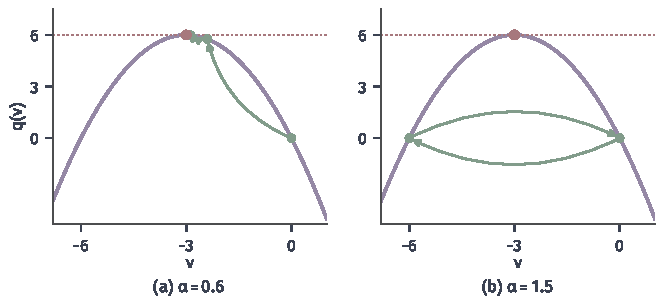
\includegraphics[width=112mm]{figures/05-optimization/06-constrained-optimization/matplotlib/pm-dual-ascent/figure.pdf}
  \caption{二元例中对偶函数$q(\nu)$（紫）上的对偶上升。绿点和箭头是乘子序列，从$\nu^{(0)}=0$出发，红点是最大点，红色点线是$f^\star=6$。(a)$\alpha=0.6$：压缩因子$0.2$，很快接近最大点。(b)$\alpha=1.5$：在$0$与$-6$之间反复跳动，不收敛。}
  \label{fig:pm-dual-ascent}
\end{BookInlineFigure}

\paragraph{可微的情形}
例子中的$q$是光滑的，这并非偶然。当$f$强凸、约束仿射时，子问题的解唯一，超梯度也唯一，对偶函数可以用第~\ref{chap:smooth-foundations}章的光滑分析。

\begin{theorem}[强凸目标的光滑对偶]
\label{thm:pm-smooth-dual}
设$f$连续可微且$\mu$强凸，$\bm{X}=\mathbb{R}^n$，约束为$\bm{A}\bm{x}=\bm{b}$。记$\bm{x}(\bm{\nu})$为$\mathcal{L}(\cdot,\bm{\nu})$的唯一最小点。则$q$可微，并且
\begin{equation}
 \nabla q(\bm{\nu})=\bm{A}\bm{x}(\bm{\nu})-\bm{b},
 \label{eq:pm-smooth-dual}
\end{equation}
其梯度满足
\begin{equation}
 \lVert\nabla q(\bm{\nu}_1)-\nabla q(\bm{\nu}_2)\rVert_2\leq\frac{\lVert\bm{A}\rVert_2^2}{\mu}\lVert\bm{\nu}_1-\bm{\nu}_2\rVert_2 .
 \label{eq:pm-smooth-dual-lipschitz}
\end{equation}
于是只要最优乘子存在，固定步长$0<\alpha<2\mu/\lVert\bm{A}\rVert_2^2$的对偶上升满足$q(\bm{\nu}^{(t)})\to d^\star$，其中$d^\star$是对偶最优值。
\end{theorem}

\begin{proof}
记$\bm{x}_k=\bm{x}(\bm{\nu}_k)$。驻定条件给出$\nabla f(\bm{x}_k)=-\bm{A}^\top\bm{\nu}_k$。由强凸性，
\[
 \mu\lVert\bm{x}_1-\bm{x}_2\rVert_2^2\leq\langle\nabla f(\bm{x}_1)-\nabla f(\bm{x}_2),\bm{x}_1-\bm{x}_2\rangle .
\]
把驻定条件代入，并用Cauchy--Schwarz不等式，得到
\[
 \mu\lVert\bm{x}_1-\bm{x}_2\rVert_2^2
 \leq-\langle\bm{\nu}_1-\bm{\nu}_2,\bm{A}(\bm{x}_1-\bm{x}_2)\rangle
 \leq\lVert\bm{A}\rVert_2\lVert\bm{\nu}_1-\bm{\nu}_2\rVert_2\lVert\bm{x}_1-\bm{x}_2\rVert_2 .
\]
两边约去一个因子，得到
\[
 \lVert\bm{x}_1-\bm{x}_2\rVert_2\leq\frac{\lVert\bm{A}\rVert_2}{\mu}\lVert\bm{\nu}_1-\bm{\nu}_2\rVert_2 .
\]

记$\bm{s}(\bm{\nu})=\bm{A}\bm{x}(\bm{\nu})-\bm{b}$。由上式，$\bm{s}$满足式~\eqref{eq:pm-smooth-dual-lipschitz}的Lipschitz界。

由定理~\ref{thm:pm-residual-supergradient}，$\bm{s}(\bm{\nu}_1)$和$\bm{s}(\bm{\nu}_2)$分别是两点的超梯度。对两点分别写一次超梯度不等式，得到
\[
 \langle\bm{s}(\bm{\nu}_2),\bm{\nu}_2-\bm{\nu}_1\rangle\leq q(\bm{\nu}_2)-q(\bm{\nu}_1)\leq\langle\bm{s}(\bm{\nu}_1),\bm{\nu}_2-\bm{\nu}_1\rangle .
\]
上下两端相差不超过$\lVert\bm{s}(\bm{\nu}_2)-\bm{s}(\bm{\nu}_1)\rVert_2\lVert\bm{\nu}_2-\bm{\nu}_1\rVert_2$，这是$\lVert\bm{\nu}_2-\bm{\nu}_1\rVert_2$的二阶量，所以$q$在$\bm{\nu}_1$处可微，梯度是$\bm{s}(\bm{\nu}_1)$。

最后，$-q$是光滑凸函数，步长范围内的梯度法收敛结论见第~\ref{chap:smooth-foundations}章和第~\ref{chap:first-order-methods}章。
\end{proof}

在二元例中，$\bm{A}=(1,1)$，$\lVert\bm{A}\rVert_2^2=2$，$f$的强凸常数$\mu=1$，定理的步长上限是$1$，比实际范围$\tfrac32$保守。这是因为定理把两个坐标方向的曲率都按最小值$\mu=1$估计，而实际的$\lvert q''\rvert$只有$\tfrac43$。

\paragraph{不可微的情形}
$f$不强凸时，子问题的解可能不唯一，$q$在这些点上有折角。下面的例子有两个变量和一条资源约束，后面还要继续使用：
\begin{equation}
 \min_{\bm{x}\in[0,1]^2}\ -x_1-x_2\qquad\text{s.t.}\qquad 2x_1+2x_2\leq3 .
 \label{eq:pm-lp-resource}
\end{equation}
它的最优值$f^\star=-1.5$，在$x_1+x_2=1.5$的线段上取得。固定$\lambda\geq0$，子问题对两个变量是分开的线性函数，每个变量的系数是$2\lambda-1$。

因此$\lambda<\tfrac12$时解是$(1,1)$，$\lambda>\tfrac12$时解是$(0,0)$，$\lambda=\tfrac12$时任意点都是解。代入得到对偶函数：
\[
 q(\lambda)=\begin{cases}\lambda-2,&\lambda\leq\tfrac12,\\-3\lambda,&\lambda\geq\tfrac12.\end{cases}
\]
$q$在$\lambda^\star=\tfrac12$处达到最大值$-1.5$，折角正好在最优点上。

超梯度步未必提高$q$。取$\alpha=0.12$，$\lambda^{(0)}=0$，乘子序列是
\[
 0,\ 0.12,\ 0.24,\ 0.36,\ 0.48,\ 0.60,\ 0.24,\ 0.36,\ 0.48,\ 0.60,\ldots
\]
对偶值$q(0.48)=-1.52$，下一步$q(0.60)=-1.8$，反而下降了。这与第~\ref{chap:nonsmooth-composite-optimization}章的次梯度法一样：步子越过折角就会下降，能保证的是到最优乘子的距离或者最好点的对偶值，而不是每步上升。图~\ref{fig:pm-primal-recovery}(a)中的绿点就在折角两侧来回。

\subsection{对偶分解与原始恢复}
\label{sec:pm-decomposition}

这一小节回答两个问题：对偶上升的计算好在哪里，以及算到最后怎样得到一个能用的原始解。

\paragraph{固定价格后各块分离}
设变量分成$K$块，目标按块可分，只有一条线性资源约束把它们联系起来：
\begin{equation}
 \min_{\bm{x}_k\in\bm{X}_k}\ \sum_{k=1}^Kf_k(\bm{x}_k)\qquad\text{s.t.}\qquad\sum_{k=1}^K\bm{A}_k\bm{x}_k\leq\bm{b}.
 \label{eq:pm-separable}
\end{equation}
固定乘子$\bm{\lambda}\geq\bm{0}$，Lagrange函数按块拆开：
\[
 \mathcal{L}(\bm{x},\bm{\lambda})=\sum_{k=1}^K\Bigl(f_k(\bm{x}_k)+\langle\bm{\lambda},\bm{A}_k\bm{x}_k\rangle\Bigr)-\langle\bm{\lambda},\bm{b}\rangle .
\]
和式中的每一项只含一块变量，所以$K$个子问题可以独立求解，互不通信。这种做法称为\term{对偶分解}（dual decomposition）。

协调者只做一件事：收集各块的用量$\bm{A}_k\bm{x}_k$，算出总残差，按下式更新价格：
\begin{equation}
 \bm{\lambda}^{(t+1)}=\Bigl[\bm{\lambda}^{(t)}+\alpha^{(t)}\Bigl(\sum_{k=1}^K\bm{A}_k\bm{x}_k^{(t)}-\bm{b}\Bigr)\Bigr]_+ .
 \label{eq:pm-decomposition-update}
\end{equation}
图~\ref{fig:pm-decomposition}以二元例为例，它本身就是两块问题：每家工厂只知道自己的成本和价格，协调者只知道总量和目标。

\begin{BookInlineFigure}
  \centering
  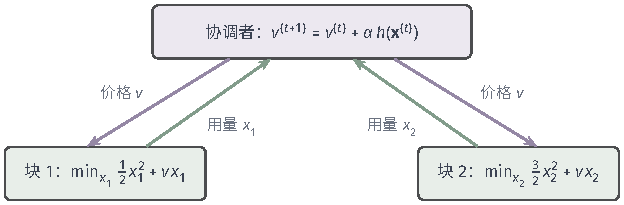
\includegraphics[width=105mm]{figures/05-optimization/06-constrained-optimization/tikz/pm-decomposition/figure.pdf}
  \caption{二元例的对偶分解。协调者（紫框）把当前价格$\nu$发给各块（紫色箭头），两块（绿框）独立求解自己的子问题，再把用量报回（绿色箭头）。协调者只用总量更新价格，不需要知道各块的成本函数。}
  \label{fig:pm-decomposition}
\end{BookInlineFigure}

分解改变的是计算的组织方式，算法在数学上仍是同一个对偶上升。收敛性质不因为分块而变好，第~\ref{chap:block-optimization}章处理的是目标本身不可分的分块，这里的分块靠乘子把约束解开。

\paragraph{原始点不可行}
继续看式~\eqref{eq:pm-lp-resource}。两个变量的子问题总是给出$(1,1)$或$(0,0)$。前者违反资源约束，$2x_1+2x_2=4>3$；后者可行，目标值却是$0$，离$f^\star$很远。图~\ref{fig:pm-primal-recovery}(b)的绿线就是这种情况：总量$x_1+x_2$一直在$2$和$0$之间跳，从不等于最优所需的$1.5$。

原因在于，对偶上升求的是价格，给定价格之后，解可以停在子问题解集的任何一点上。这个例子里，$\lambda^\star=\tfrac12$处的子问题有无穷多解，$q$的最大点却完全不告诉我们选哪个。

\paragraph{平均恢复}
第~\ref{chap:nonsmooth-composite-optimization}章在次梯度法上用过的平均，这里有直接的物理含义。把$\lambda$上涨的轮次看成资源用多了，下跌的轮次看成用少了，平均之后用量大致等于资源总量。图~\ref{fig:pm-primal-recovery}(b)的黄线是$x_1^{(t)}+x_2^{(t)}$的累积平均，它趋于$1.5$。

\begin{BookInlineFigure}
  \centering
  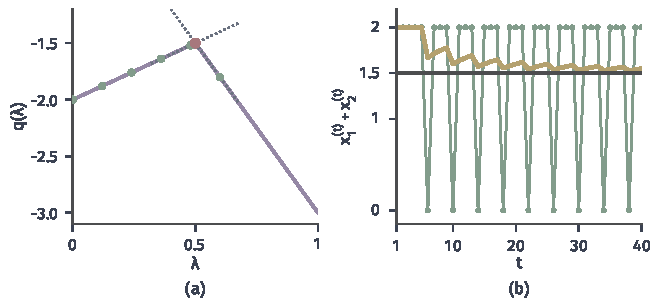
\includegraphics[width=112mm]{figures/05-optimization/06-constrained-optimization/matplotlib/pm-primal-recovery/figure.pdf}
  \caption{资源问题的超梯度上升，$\alpha=0.12$。(a)紫线是对偶函数，折角在$\lambda^\star=\tfrac12$，灰色点线是折角处的两条支撑线，绿点是前九个乘子，红点是最大点。(b)绿线是每轮的总量$x_1^{(t)}+x_2^{(t)}$，在$2$与$0$之间跳动；黄线是累积平均，深灰线是$1.5$。}
  \label{fig:pm-primal-recovery}
\end{BookInlineFigure}

\begin{theorem}[平均点的可行性与目标]
\label{thm:pm-primal-average}
设$f$和$g_i$在非空紧凸集$\bm{X}$上凸且连续，问题只有不等式约束，$f^\star$有限。设$\lVert\bm{g}(\bm{x})\rVert_2\leq S$对$\bm{x}\in\bm{X}$成立。从$\bm{\lambda}^{(0)}\geq\bm{0}$出发，取固定步长$\alpha>0$运行式~\eqref{eq:pm-dual-ascent}。记$\bar{\bm{x}}^{(T)}$为$\bm{x}^{(0)},\ldots,\bm{x}^{(T-1)}$的算术平均，则平均点在$\bm{X}$内，并且
\begin{equation}
 \bm{g}(\bar{\bm{x}}^{(T)})\leq\frac{\bm{\lambda}^{(T)}}{\alpha T},
 \label{eq:pm-average-feasibility}
\end{equation}
\begin{equation}
 f(\bar{\bm{x}}^{(T)})-f^\star\leq\frac{\lVert\bm{\lambda}^{(0)}\rVert_2^2}{2\alpha T}+\frac{\alpha S^2}{2}.
 \label{eq:pm-average-objective}
\end{equation}
\end{theorem}

\begin{proof}
先证可行性。投影只会让乘子变大，$[a]_+\geq a$，所以
\[
 \bm{\lambda}^{(t+1)}\geq\bm{\lambda}^{(t)}+\alpha\bm{g}(\bm{x}^{(t)}).
\]
对$t=0,\ldots,T-1$求和，得到
\[
 \alpha\sum_{t=0}^{T-1}\bm{g}(\bm{x}^{(t)})\leq\bm{\lambda}^{(T)}-\bm{\lambda}^{(0)}\leq\bm{\lambda}^{(T)}.
\]
每个$g_i$是凸函数，由Jensen不等式，平均点上的函数值不超过函数值的平均：
\[
 g_i(\bar{\bm{x}}^{(T)})\leq\frac1T\sum_{t=0}^{T-1}g_i(\bm{x}^{(t)}).
\]
两式结合，除以$\alpha T$，即得式~\eqref{eq:pm-average-feasibility}。

再证目标。投影到非负象限不增加与原点的距离，所以
\[
 \lVert\bm{\lambda}^{(t+1)}\rVert_2^2\leq\lVert\bm{\lambda}^{(t)}+\alpha\bm{g}(\bm{x}^{(t)})\rVert_2^2\leq\lVert\bm{\lambda}^{(t)}\rVert_2^2+2\alpha\langle\bm{\lambda}^{(t)},\bm{g}(\bm{x}^{(t)})\rangle+\alpha^2S^2 .
\]
由弱对偶和$\bm{x}^{(t)}$的定义，
\[
 f(\bm{x}^{(t)})+\langle\bm{\lambda}^{(t)},\bm{g}(\bm{x}^{(t)})\rangle=q(\bm{\lambda}^{(t)})\leq f^\star .
\]
从上式解出内积，代入前一个不等式，得到
\[
 f(\bm{x}^{(t)})-f^\star\leq\frac{\lVert\bm{\lambda}^{(t)}\rVert_2^2-\lVert\bm{\lambda}^{(t+1)}\rVert_2^2}{2\alpha}+\frac{\alpha S^2}{2}.
\]
对$t$求和，左边用Jensen不等式，右边裂项相消，去掉非正的$-\lVert\bm{\lambda}^{(T)}\rVert_2^2$，除以$T$即得式~\eqref{eq:pm-average-objective}。
\end{proof}

平均点的违规量由$\bm{\lambda}^{(T)}/(\alpha T)$控制，只要乘子序列有界，它就以$1/T$趋于零。Slater条件可以保证有界。设$\tilde{\bm{x}}\in\bm{X}$满足$g_i(\tilde{\bm{x}})\leq-\sigma<0$，并记$f_{\min}$为$f$在$\bm{X}$上的最小值。对偶函数不超过$\mathcal{L}$在$\tilde{\bm{x}}$处的值，由此得到
\[
 \langle\bm{\lambda}^{(t)},\bm{g}(\bm{x}^{(t)})\rangle=q(\bm{\lambda}^{(t)})-f(\bm{x}^{(t)})\leq f(\tilde{\bm{x}})-f_{\min}-\sigma\lVert\bm{\lambda}^{(t)}\rVert_1 .
\]
记
\[
 R=\frac{f(\tilde{\bm{x}})-f_{\min}+\alpha S^2/2}{\sigma}.
\]
代入证明中的距离递推可知，只要$\lVert\bm{\lambda}^{(t)}\rVert_1\geq R$，范数就不会增大；否则一步至多增加$\alpha S$。所以
\[
 \lVert\bm{\lambda}^{(t)}\rVert_2\leq\max\bigl\{\lVert\bm{\lambda}^{(0)}\rVert_2,\ R+\alpha S\bigr\}.
\]

式~\eqref{eq:pm-average-objective}只是单侧的界：$\bar{\bm{x}}^{(T)}$略微不可行时，目标值可能低于$f^\star$。

在问题~\eqref{eq:pm-lp-resource}中，乘子进入周期后每四轮有三轮是$(1,1)$，一轮是$(0,0)$，平均趋于$(\tfrac34,\tfrac34)$，$2x_1+2x_2$趋于$3$，恰好用尽资源。这组权重$\tfrac34,\tfrac14$是从对偶迭代的频率里读出来的，并没有事先知道。

\paragraph{非凸时的恢复与证书}
平均依赖可行集和目标的凸性。把式~\eqref{eq:pm-lp-resource}的变量改成$x_i\in\{0,1\}$，子问题和对偶函数都不变，最优乘子仍是$\tfrac12$，下界最多是$-1.5$。可平均点$(\tfrac34,\tfrac34)$不是整数点，平均在这里没有意义。

这时可以从访问过的点里挑选，或者另加一个简单的修复步骤，例如按边际价值贪心地放入物品，直到资源用尽。这里贪心得到$(1,0)$，目标值$-1$，可行。

此时的结论要如实报告：可行解给出上界$-1$，迭代中最好的对偶值给出下界$-1.52$，间隙不超过$0.52$。这个问题真实的最优值是$-1$，对偶下界不紧是非凸问题的常态，第~\ref{chap:duality}章称之为对偶间隙。任何情况下都应当同时报告原始可行性和这个间隙，单独一个收敛的对偶值不构成原问题的解。
